\PassOptionsToPackage{unicode=true}{hyperref} % options for packages loaded elsewhere
\PassOptionsToPackage{hyphens}{url}
%
\documentclass[]{article}
\usepackage{lmodern}
\usepackage{amssymb,amsmath}
\usepackage{ifxetex,ifluatex}
\usepackage{fixltx2e} % provides \textsubscript
\ifnum 0\ifxetex 1\fi\ifluatex 1\fi=0 % if pdftex
  \usepackage[T1]{fontenc}
  \usepackage[utf8]{inputenc}
  \usepackage{textcomp} % provides euro and other symbols
\else % if luatex or xelatex
  \usepackage{unicode-math}
  \defaultfontfeatures{Ligatures=TeX,Scale=MatchLowercase}
\fi
% use upquote if available, for straight quotes in verbatim environments
\IfFileExists{upquote.sty}{\usepackage{upquote}}{}
% use microtype if available
\IfFileExists{microtype.sty}{%
\usepackage[]{microtype}
\UseMicrotypeSet[protrusion]{basicmath} % disable protrusion for tt fonts
}{}
\IfFileExists{parskip.sty}{%
\usepackage{parskip}
}{% else
\setlength{\parindent}{0pt}
\setlength{\parskip}{6pt plus 2pt minus 1pt}
}
\usepackage{hyperref}
\hypersetup{
            pdfborder={0 0 0},
            breaklinks=true}
\urlstyle{same}  % don't use monospace font for urls
\usepackage{graphicx,grffile}
\makeatletter
\def\maxwidth{\ifdim\Gin@nat@width>\linewidth\linewidth\else\Gin@nat@width\fi}
\def\maxheight{\ifdim\Gin@nat@height>\textheight\textheight\else\Gin@nat@height\fi}
\makeatother
% Scale images if necessary, so that they will not overflow the page
% margins by default, and it is still possible to overwrite the defaults
% using explicit options in \includegraphics[width, height, ...]{}
\setkeys{Gin}{width=\maxwidth,height=\maxheight,keepaspectratio}
\setlength{\emergencystretch}{3em}  % prevent overfull lines
\providecommand{\tightlist}{%
  \setlength{\itemsep}{0pt}\setlength{\parskip}{0pt}}
\setcounter{secnumdepth}{0}
% Redefines (sub)paragraphs to behave more like sections
\ifx\paragraph\undefined\else
\let\oldparagraph\paragraph
\renewcommand{\paragraph}[1]{\oldparagraph{#1}\mbox{}}
\fi
\ifx\subparagraph\undefined\else
\let\oldsubparagraph\subparagraph
\renewcommand{\subparagraph}[1]{\oldsubparagraph{#1}\mbox{}}
\fi

% set default figure placement to htbp
\makeatletter
\def\fps@figure{htbp}
\makeatother


\date{}

\begin{document}

\hypertarget{projecte-asix-2k22}{%
\section{\texorpdfstring{\textbf{Projecte ASIX
2k22}}{Projecte ASIX 2k22}}\label{projecte-asix-2k22}}

\hypertarget{escola-del-treball}{%
\subsection{\texorpdfstring{\textbf{Escola Del
Treball}}{Escola Del Treball}}\label{escola-del-treball}}

\hypertarget{hisx-2021-2022}{%
\subsubsection{\texorpdfstring{\textbf{2HISX
2021-2022}}{2HISX 2021-2022}}\label{hisx-2021-2022}}

\hypertarget{aaron-andal-cristian-condolo}{%
\subsubsection{\texorpdfstring{\textbf{Aaron Andal \& Cristian
Condolo}}{Aaron Andal \& Cristian Condolo}}\label{aaron-andal-cristian-condolo}}

\hypertarget{cryptosec-careful-where-you-step-in}{%
\section{\texorpdfstring{\textbf{CryptoSEC}: ``\emph{Careful where you
step
in}''}{CryptoSEC: ``Careful where you step in''}}\label{cryptosec-careful-where-you-step-in}}

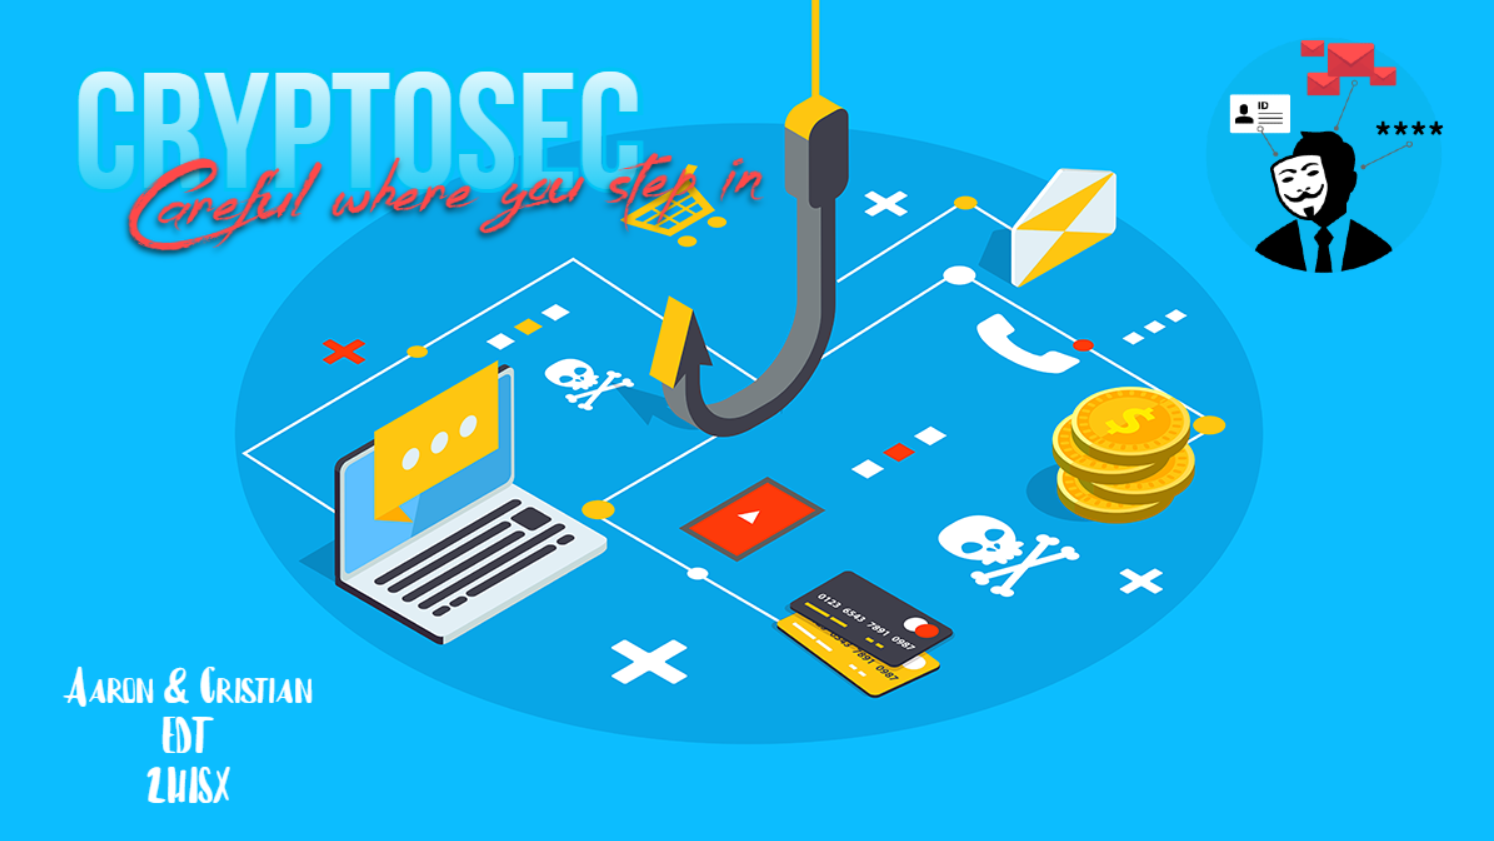
\includegraphics{./tex2pdf.-daaaa42b20fc4097/785b57206d80bd3d5ef15f036481e103db8435a1.png}

\hypertarget{index}{%
\section{\texorpdfstring{\textbf{Index}}{Index}}\label{index}}

\begin{itemize}
\item
  \textbf{Bettercap}: \protect\hyperlink{bettercap}{--\textgreater{}
  readME \textless{}--}
\item
  \textbf{Carecterístiques de Bettercap}:
  \protect\hyperlink{carecteruxedstiques-de-bettercap}{--\textgreater{}
  readME \textless{}--}

  \begin{itemize}
  \item
    \textbf{Eavesdropping (Escoltar atentament)}:
    \protect\hyperlink{eavesdropping-escoltar-atentament}{--\textgreater{}
    readME \textless{}--}
  \item
    \textbf{Falsificació de direccions IP (Address Spoofing o DNS Cache
    Poisoning + ARP Spoof)}:
    \protect\hyperlink{falsificaciuxf3-de-direccions-ip-address-spoofing-o-dns-cache-poisoning--arp-spoof}{--\textgreater{}
    readME \textless{}--}
  \item
    \textbf{Atac de denegació de servei (DoS)}:
    \protect\hyperlink{atac-de-denegaciuxf3-de-servei-dos}{--\textgreater{}
    readME \textless{}--}
  \item
    \textbf{Atac Man in the Middle}:
    \protect\hyperlink{atac-man-in-the-middle}{--\textgreater{} readME
    \textless{}--}
  \end{itemize}
\item
  \textbf{Exemple pràctic d'Ettercap}:
  \protect\hyperlink{exemple-pruxe0ctic-dettercap}{--\textgreater{}
  readME \textless{}--}

  \begin{itemize}
  \item
    \textbf{Exemple utilitzant \textbf{setoolkit} a Kali Linux i
    ETTERCAP}:
    \protect\hyperlink{exemple-1-utilitzant-setoolkit-a-kali-linux-i-ettercap}{--\textgreater{}
    readME \textless{}--}
  \item
    \textbf{Explicació resumida}:
    \protect\hyperlink{explicaciuxf3-resumida}{--\textgreater{} readME
    \textless{}--}
  \end{itemize}
\item
  \textbf{Bibliografia}:
  \protect\hyperlink{bibliografia}{--\textgreater{} readME
  \textless{}--}
\end{itemize}

\hypertarget{bettercap}{%
\section{\texorpdfstring{\textbf{Bettercap}}{Bettercap}}\label{bettercap}}

\textbf{BetterCAP} és una eina potent, flexible i portàtil creada per
realitzar diversos tipus datacs MITM contra una xarxa, manipular HTTP,
HTTPS i trànsit TCP en temps real, buscar credencials i molt més.
Analitzador de xarxa via web; inclou BlueTooth, Wifi , Detecta atacs
MITM , Spoof, network protocol fuzzer

\includegraphics{./tex2pdf.-daaaa42b20fc4097/36eb054d18ec1a19cb60c01aeef47ee0d9c67d6d.jpg}

Bettercap està escrit en codi Ruby i s'aprofita de la flexibilitat i el
potencial d'aquest llenguatge.

La instal·lació de Bettercap és realment senzilla. Té dependències, però
executant gem install bettercap el procés es duu a terme completament.
En cas que necessiteu alguna llibreria es pot utilitzar apt-get per
completar el procés. Un cop instal·lat, disposarem d'un binari, el qual
podrem executar.

\hypertarget{carecteruxedstiques-de-bettercap}{%
\section{\texorpdfstring{\textbf{Carecterístiques de
Bettercap}}{Carecterístiques de Bettercap}}\label{carecteruxedstiques-de-bettercap}}

Bettercap és una eina molt potent que és compatible amb les principals
distribucions basades en Linux, algunes de les seves característiques
principals són les següents:

\begin{itemize}
\item
  Escàner de xarxes WiFi , permet fer atacs de desautotenticació, també
  permet realitzar atacs sense clients a associacions PMKID, permet
  capturar handshakes de clients que usen protocol WPA i WPA2.
\item
  Escàner de dispositius BLE ( Bluetooth Low Energia) per llegir i
  escriure informació.
\item
  Escàner de dispositius sense fil que usin la banda de 2.4GHz, com els
  ratolins sense fil, també permet realitzar atacs MouseJacking amb
  injecció de dades.
\item
  Permet fer atacs passius i actius a xarxes IP
\item
  Permet fer atacs MitM basats en ARP, DNS i també DHCPv6, amb
  l'objectiu de capturar tota la informació.
\item
  Permet crear un servidor intermediari HTTP/HTTPS per aixecar el
  trànsit segur HTTPS, i facilita enormement l'ús de scripts.
\item
  Sniffer de xarxa molt potent per a recol·lecció de credencials
  dusuari.
\item
  Escàner de ports molt ràpid
\item
  Té una potent API REST per fer atacs fàcilment.
\item
  Incorpora una interfície gràfica d'usuari per facilitar els atacs,
  encara que el terminal de comandaments és molt potent.
\item
  Tenim una gran quantitat de mòduls de diferents categories per ampliar
  funcionalitats
\end{itemize}

\hypertarget{els-atacs-que-es-poden-fer-a-bettercap}{%
\section{\texorpdfstring{\textbf{Els atacs que es poden fer a
Bettercap}}{Els atacs que es poden fer a Bettercap}}\label{els-atacs-que-es-poden-fer-a-bettercap}}

\hypertarget{eavesdropping-escoltar-atentament}{%
\subsection{\texorpdfstring{\textbf{Eavesdropping (Escoltar
atentament)}}{Eavesdropping (Escoltar atentament)}}\label{eavesdropping-escoltar-atentament}}

Segur que et resulta familiar; és una cosa molt normal a la vida.
Imagina't que vols trobar alguna informació sobre dos amics i la seva
relació. Una manera molt senzilla és escoltar en secret les vostres
paraules. Aquest tipus d'atac també es produeix a les comunicacions
informàtiques, però es coneix com a \textbf{sniffing}.

\includegraphics{./tex2pdf.-daaaa42b20fc4097/193c2dd9e32f432bea47a8c10364a792fbb446d8.jpg}

Quan xateges amb el teu amic en mode ``text clar'', és possible olorar
el teu trànsit. Pot semblar antic, però pots estar segur que és un dels
problemes de seguretat més grans en una xarxa que els administradors de
xarxa no tenen en compte.

\hypertarget{falsificaciuxf3-de-direccions-ip-address-spoofing-o-dns-cache-poisoning-arp-spoof}{%
\subsection{\texorpdfstring{\textbf{Falsificació de direccions IP
(Address Spoofing o DNS Cache Poisoning + ARP
Spoof)}}{Falsificació de direccions IP (Address Spoofing o DNS Cache Poisoning + ARP Spoof)}}\label{falsificaciuxf3-de-direccions-ip-address-spoofing-o-dns-cache-poisoning-arp-spoof}}

Sé que saps què és una adreça IP (Protocol d'Internet). Com saps, per
comunicar-se amb altres ordinadors, cada ordinador necessita una IP. En
aquest atac, un atacant vol fer una adreça de destinació falsa i
enganyar-te sobre això. Per exemple, el teu objectiu és mibanco.com i un
atacant reenvia la teva petició a un fals mibanco.com. L'objectiu és
suplantar el host víctima.

\includegraphics{./tex2pdf.-daaaa42b20fc4097/4e2192effcf29c7836c29ece4a04b8ab2875d519.1}

\hypertarget{atac-de-denegaciuxf3-de-servei-dos}{%
\subsection{\texorpdfstring{\textbf{Atac de denegació de servei
(DoS)}}{Atac de denegació de servei (DoS)}}\label{atac-de-denegaciuxf3-de-servei-dos}}

En aquest tipus d'atac, un atacant intenta fer que una màquina o un
recurs de xarxa no estigui disponible per als usuaris.

L'objectiu és interrompre o suspendre els serveis que es connecten a
Internet. Aquest atac es dirigeix ​​a gateways i servidors web, com els
dels bancs, i realitza alguns dels sabotatges següents.

\begin{itemize}
\item
  Ús de recursos computacionals, com lample de banda, la memòria, lespai
  en disc o fins i tot la CPU. Com suposo, la teva ment podria divagar
  cap al codi maliciós.
\item
  Destrueix la informació i les taules d'encaminament.
\item
  Interrompre els components físics de la xarxa, com els routers, els
  switches i els firewalls.
\item
  Envia dades no vàlides a aplicacions o serveis de xarxa. Podeu acabar
  anormalment els serveis.
\item
  Enviar molts paquets a les destinacions per inundar-los i finalment
  col·lapsar i apagar.
\item
  Bloquejar les destinacions i que els usuaris autoritzats no hi puguin
  accedir.
\end{itemize}

Al DDoS, un atacant pot utilitzar la tècnica del Zombie per capturar
molts ordinadors i enviar moltes peticions a la víctima a través d'ells
o de bots. Zombie vol dir que un ordinador connectat a Internet ha estat
compromès per un hacker.

\includegraphics{./tex2pdf.-daaaa42b20fc4097/b11d3d9883292ce939094fc1aa96ac0d3d072c3d.png}

\hypertarget{atac-man-in-the-middle}{%
\subsection{\texorpdfstring{\textbf{Atac Man in the
Middle}}{Atac Man in the Middle}}\label{atac-man-in-the-middle}}

L'atac man-in-the-middle (abreujat MITM, MitM, MIM, MiM, MITMA) és una
forma d'atac actiu en què un atacant estableix una connexió entre les
víctimes i envia missatges entre elles.

Així, les víctimes creuen que estan parlant directament entre elles,
però en realitat un atacant ho controla.

En aquest escenari, un atacant ha tingut èxit quan es pot fer passar per
un usuari.

D'altra banda, hi ha una tercera persona entre tu i la persona amb qui
et comuniques i pot controlar i vigilar el teu trànsit.

\includegraphics{./tex2pdf.-daaaa42b20fc4097/e98cb868fc160cd04f0803fecc4eb4d2ba9a8069.png}

Afortunadament, alguns protocols poden impedir-ho, com el SSL.

Un hacker pot utilitzar el següent programari per implementar aquest
atac:

\begin{itemize}
\item
  Caín i Abel
\item
  Subterfugi
\item
  \textbf{Ettercap}: És el que utilitzarem
\item
  AirJack
\item
  \textbf{SSLStrip}: L'utilitzarem per trencar el SSL.
\item
  \textbf{SSLSniff}
\end{itemize}

\hypertarget{exemple-pruxe0ctic-de-bettercap}{%
\section{\texorpdfstring{\textbf{Exemple pràctic de
BETTERCAP}}{Exemple pràctic de BETTERCAP}}\label{exemple-pruxe0ctic-de-bettercap}}

\hypertarget{arp-poisoning-spoofing-en-acciuxf3}{%
\section{\texorpdfstring{\textbf{ARP Poisoning / Spoofing en
acció}}{ARP Poisoning / Spoofing en acció}}\label{arp-poisoning-spoofing-en-acciuxf3}}

\hypertarget{arp-poisoning-spoofing-2-parts-bettercap}{%
\subsection{\texorpdfstring{\textbf{ARP Poisoning / Spoofing (2 parts)
(BETTERCAP)}:}{ARP Poisoning / Spoofing (2 parts) (BETTERCAP):}}\label{arp-poisoning-spoofing-2-parts-bettercap}}

Envenenament de les taules ARP de les víctimes implicades i reenviament
de paquets al hacker. Amb el Wireshark - ARP - Nmap, veurem com fa el
duplicat de MAC.

\includegraphics{./tex2pdf.-daaaa42b20fc4097/e3bfba9a468da065f52920b3855d57ead71eb82c.png}

\includegraphics{./tex2pdf.-daaaa42b20fc4097/812210a5f20009ba736a6bc20baa9e7706a123fc.png}

\hypertarget{mitm---eavesdropping-sniffing-bettercap}{%
\subsubsection{\texorpdfstring{\textbf{MITM - Eavesdropping (Sniffing)
(BETTERCAP)}}{MITM - Eavesdropping (Sniffing) (BETTERCAP)}}\label{mitm---eavesdropping-sniffing-bettercap}}

Amb l'ARP Poisoning d'abans activarem un \emph{sniffer} i estarem
escoltant la màquina afectada i veient les pàgines on visita. Podem
captar credencials de pàgines HTTP.

\begin{enumerate}
\def\labelenumi{\arabic{enumi}.}
\item
  Obrir el Bettercap a Kali Linux.
\item
  Tenim una interfície senzilleta per començar a fer l'atac Man in the
  Middle. Si fem `\texttt{help} podrem veure tots els mòduls
  disponibles.
\end{enumerate}

\includegraphics{./tex2pdf.-daaaa42b20fc4097/df9380df862264ed5291ba883e42022c1ba9b4fe.png}

\begin{enumerate}
\def\labelenumi{\arabic{enumi}.}
\setcounter{enumi}{1}
\tightlist
\item
  Amb la comanda següent \texttt{net.show} ens mostrarà la IP - MAC -
  Nom local. Seguidament fem un \texttt{net.probe\ on} per observar de
  forma interactiva i per fer-ho més bonic, amb un \texttt{ticker\ on}
\end{enumerate}

\includegraphics{./tex2pdf.-daaaa42b20fc4097/4713ed44f6cee026b98209ea83df9560e03f4dac.png}

\includegraphics{./tex2pdf.-daaaa42b20fc4097/06a817aaae7be8d48fe97574a6ae6fa98a95373b.png}

\includegraphics{./tex2pdf.-daaaa42b20fc4097/92504a7d13d33df8a8da22e221b47b82e6d7845d.png}

\includegraphics{./tex2pdf.-daaaa42b20fc4097/e66adb6d51103780f2c8524fb521bc5e3bd9a25a.png}

\begin{enumerate}
\def\labelenumi{\arabic{enumi}.}
\setcounter{enumi}{2}
\tightlist
\item
  A partir d'aquest moment, quan ja hem escollit la IP de la víctima. Ja
  podem començar amb el ARP.SPOOF
\end{enumerate}

\includegraphics{./tex2pdf.-daaaa42b20fc4097/46712dbb6a0bab4b7678601b9408dd08d371b3c1.png}

\includegraphics{./tex2pdf.-daaaa42b20fc4097/11d58511333c2068444688bb8b0728c225ecb7fd.png}

\includegraphics{./tex2pdf.-daaaa42b20fc4097/7fffb68e3e33e5688375ebfd87d43ed69feb31f7.png}

\includegraphics{./tex2pdf.-daaaa42b20fc4097/c9f979cba96be2e9f55372aaef6720a8647d36f6.png}

\hypertarget{dns-poisoning-spoofing-bettercap}{%
\subsubsection{\texorpdfstring{\textbf{DNS Poisoning / Spoofing)
(BETTERCAP)}}{DNS Poisoning / Spoofing) (BETTERCAP)}}\label{dns-poisoning-spoofing-bettercap}}

Amb l'ARP Spoof d'abans activarem un \emph{dnsspoof} i injectarem un
registre de DNS fals on ens redirigirà a la nostra màquina on hi tindrem
una \emph{fake page: m0odle.escoladeltreball.org} (\textbf{Moodle EDT})
i l'enviarem per correu utilitzant \textbf{SET} dient que
``\emph{URGENT! L'Eduard ha posat les notes de M06, entra urgentment i
mira la nota que tens!!!}'' llavors l'usuari entrarà i no se n'adonarà i
li robarem les credencials mostrades al \textbf{SET}.

\includegraphics{./tex2pdf.-daaaa42b20fc4097/e3327f607e33f9c2b9ebb1b8fcfb326a26032794.png}

\includegraphics{./tex2pdf.-daaaa42b20fc4097/1de4d8ed3f6bd95797e9a4a6d79391b639801263.png}

\includegraphics{./tex2pdf.-daaaa42b20fc4097/38e1a84c34d0f52ad7f2111413dc8902b959285d.png}

\includegraphics{./tex2pdf.-daaaa42b20fc4097/55ef228ea8afa79c3d6854268f9b301c627fec7c.png}

\includegraphics{./tex2pdf.-daaaa42b20fc4097/654367c45437aa293f86a84b7c9d002b1df793da.png}

\hypertarget{a-partir-daquuxed-generem-el-mail-phishing-desde-un-compte-de-gmail-robat-a-cryptosec.}{%
\subsubsection{\texorpdfstring{A partir d'aquí generem el \textbf{mail
phishing} desde un compte de gmail robat a
\textbf{CryptoSEC}.}{A partir d'aquí generem el mail phishing desde un compte de gmail robat a CryptoSEC.}}\label{a-partir-daquuxed-generem-el-mail-phishing-desde-un-compte-de-gmail-robat-a-cryptosec.}}

\begin{enumerate}
\def\labelenumi{\arabic{enumi}.}
\tightlist
\item
  Seleccionem la opció 5: \textbf{Mass Mailer Attack}.
\end{enumerate}

\includegraphics{./tex2pdf.-daaaa42b20fc4097/6842b6f01f25b6f2ff37aaa977f1ea8c997dbc42.png}

\begin{enumerate}
\def\labelenumi{\arabic{enumi}.}
\setcounter{enumi}{1}
\tightlist
\item
  Seleccionem la opció 5: \textbf{Mass Mailer Attack}. Omplim les
  opcions: \texttt{1}, \texttt{email\ destination}, \texttt{1},
  \texttt{our\ email\ address}, \texttt{our\ email\ password},
  \texttt{priority}, \texttt{attach\ file},
  \texttt{fake\ email\ subject}, \texttt{body\ of\ messeage\ with\ END}
\end{enumerate}

\includegraphics{./tex2pdf.-daaaa42b20fc4097/7c90bc2a459ba5f1d3e62cd621f6ccccd3ee7937.png}

\includegraphics{./tex2pdf.-daaaa42b20fc4097/929927b5c6b901c64dca177f88811768f7156a5a.png}

\includegraphics{./tex2pdf.-daaaa42b20fc4097/b76a762cc63b335594c87f370e425b27344ff080.png}

\includegraphics{./tex2pdf.-daaaa42b20fc4097/42e15067e372bda97541c8e7bd31a0e19db80aa3.png}

\includegraphics{./tex2pdf.-daaaa42b20fc4097/262a9464fcab18ca95fa080d338bc060b3eaf7b5.png}

\includegraphics{./tex2pdf.-daaaa42b20fc4097/55134d95567656fb5c21b404c925b602681309ae.png}

\includegraphics{./tex2pdf.-daaaa42b20fc4097/e3ad4f17837b292d5af2b1e2dd474e24d5b9b077.png}

\hypertarget{spoofing-cryptosec.net-with-dos-attack-bettercap-slowhttp}{%
\subsection{\texorpdfstring{\textbf{Spoofing CryptoSEC.NET with DOS
Attack (BETTERCAP)
(SlowHTTP)}}{Spoofing CryptoSEC.NET with DOS Attack (BETTERCAP) (SlowHTTP)}}\label{spoofing-cryptosec.net-with-dos-attack-bettercap-slowhttp}}

Ídem que l'anterior però els targets son el \textbf{SOA} i el
\textbf{Forwarding}, els clients interns de CryptoSEC quan hagin d'anar
a la pàgina web \textbf{cryptosec.net}, entraràn a
\textbf{cryptos3c.net} ja que el hacker ha avisat que hi hà una urgència
a la pàgina principal i han d'entrar a la pàgina web dada pel hacker i
les seves credencials seràn \textbf{robades sense que se'n adoni}!

\begin{enumerate}
\def\labelenumi{\arabic{enumi}.}
\item
  El hacker activar el ARP Spoof amb targets del SOA i el Forwarder.
\item
  El hacker ha realitzat un DOS per tumbar l'apache2 (SOA):
  \texttt{hping3\ -\/-randsource\ -p80\ -S\ -\/-flood\ 10.200.243.164}
\end{enumerate}

Ara explicaré què significa cada part de l'ordre:

\begin{itemize}
\item
  \textbf{p 80} és el port que triem atacar
\item
  S activa el flag Syn
\end{itemize}

-- flood indica a hping que enviï els paquets a la màxima velocitat
possible

\begin{itemize}
\tightlist
\item
  ip\_victima és la \textbf{ip} o \textbf{domini} a atacar
\end{itemize}

Si volem que la nostra ip no sigui visible podem afegir-li l'opció --ai
la ip que falsejarem o bé utilitzar --rand-source amb què es generen
adreces d'origen ip a l'atzar:

\texttt{hping3\ -\/-randsource\ -p80\ -S\ -\/-flood\ 10.200.243.164}

o també podem utilitzar: \texttt{Slowhttptest}, nosaltres utilitzarem
\textbf{slowhttptest}.

\begin{quote}
\emph{slowhttptest - Denial Of Service attacks simulator}
\end{quote}

\texttt{slowhttptest\ -c\ 40000\ -H\ -i\ 30\ -r\ 500\ -l\ 600\ -u\ http://cryptosec.net}

\texttt{-c} \emph{number of connections Specifies the target number of
connections to establish during the test.}

\texttt{-H\textquotesingle{}} \emph{Starts slowhttptest in SlowLoris
mode, sending unfinished HTTP requests.}

\texttt{-i} \emph{seconds Specifies the interval between follow up data
for slowrois and Slow POST tests.}

\texttt{-r} \emph{connections per second Specifies the connection rate.}

\texttt{-l} \emph{seconds Specifies test duration in seconds.}

\texttt{-u} \emph{URL Specifies the URL.}

\includegraphics{./tex2pdf.-daaaa42b20fc4097/76184170fb9b877466b9abd583a6deefe121ee2d.png}

\includegraphics{./tex2pdf.-daaaa42b20fc4097/d5f88fdd642925df7b1c2c6a12628d9bcd6dc623.png}

\begin{enumerate}
\def\labelenumi{\arabic{enumi}.}
\setcounter{enumi}{1}
\tightlist
\item
  El hacker activa la pàgina del \textbf{cryptos3c.net} (fake) amb el
  SET (\textbf{Social Engineering Tool}).
\end{enumerate}

\includegraphics{./tex2pdf.-daaaa42b20fc4097/6ecb90c265f5c0262d5eedea4fd75fde5d7855f4.png}

\includegraphics{./tex2pdf.-daaaa42b20fc4097/b4519d62ff8a1231edf6f239039becd521f8bb10.png}

\includegraphics{./tex2pdf.-daaaa42b20fc4097/1b2113d36a0b18aeb905aa5e3a96e98d572f0b9d.png}

\includegraphics{./tex2pdf.-daaaa42b20fc4097/df80a6920a82363851e96ae5ecf26638d1aa88ef.png}

\begin{enumerate}
\def\labelenumi{\arabic{enumi}.}
\setcounter{enumi}{2}
\item
  El hacker emet un comunicat general a l'empresa dient que s'ha caigut
  temporalment la pàgina principal i que han d'entrar per la pàgina
  següent \texttt{cryptos3c.net}
\item
  Des d'un client de la xarxa interna de CryptoSEC 192.168.3.100
  (\emph{Linux Lite Client}) es vol conectar a la pàgina web de
  cryptosec.net, però han emès un comunicat que els redirecciona a
  \textbf{cryptos3c.net} ja que la pàgina principal ha sigut hackejada
  amb DOS (denegació de servei).
\end{enumerate}

\includegraphics{./tex2pdf.-daaaa42b20fc4097/989e8e1d4b74156442149c98e003c47e2c6033d1.png}

\begin{enumerate}
\def\labelenumi{\arabic{enumi}.}
\setcounter{enumi}{4}
\tightlist
\item
  Les credencials del client han sigut robades!
\end{enumerate}

\hypertarget{bibliografia}{%
\section{\texorpdfstring{\textbf{Bibliografia}:}{Bibliografia:}}\label{bibliografia}}

\begin{itemize}
\tightlist
\item
  https://www.redeszone.net/tutoriales/seguridad/descifrar-trafico-https-bettercap-linux/
\end{itemize}

\end{document}
